\section{Internal Processes}
Internal processes are jobs submitted to StreamFS that are written in Javascript and managed within a StreamFS cluster.

StreamFS distinguishes between nodes that represent streaming data sources in the real-world
and those that do not.  Those that do not, however, can be tagged as aggregation points.  As part of the 
tagging processes, a user specifies the units of aggregation, with additional options for cleaning
and processing.  Our contributions are:  

\begin{itemize}
\item Use of the entity-relationship graph to provide OLAP \emph{roll-up}, \emph{drill-down},
		and \emph{slice and dice} operations.
\item Show how sliding-window operations can be used on real-time data in combination with the entity-relationship
		graph to maintain accurate aggregates as the underlying objects and inter-relationships change.
\end{itemize}


% \subsection{Mapping OLAP to ERG}
\subsection{OLAP-style Aggregation}

% \begin{itemize}
% \item Introduction to OLAP.
% \item Explanation of ERG in StreamFS.
% \end{itemize}
Online analytical processing (OLAP) is a processing layer that provides summurization of data
from a set of underlying data repository (date warehouses).  Traditionally, OLAP is used to process
business data.  Business data summurization allows an analyst ask targetted questions about aggregates 
and trends in their data.  The data is typically multidimensional in nature and operations can be performed with
respect to those dimensions and their inter-relationship.

\subsubsection{Measures, Dimenions, and Levels}
Measures are the value, dimensions are the units of measure as well as time, and levels/hierarchy are 
explicit in the naming structure.

\subsubsection{Operations: drill-down and roll-up}
Drill-down and roll-up are made explicit in the structure.  You can drill down to individual readings or roll them
up into an aggregation point at a particular level in the hierarchy.

\subsubsection{Operations: slice and dice}
Slice and dice operations 

\subsubsection{Operations: pivoting}
\subsection{Dynamic Aggregation}
\label{sec:dynagg}
Dynamic aggregation combines the underlying entity-relationship graph with in-network aggregation.  It treats
each node in the graph as a potential point of aggregation on a particular data type.  For example,
if we need to compute aggregates of \emph{KW} data and we declare the node for a particular room as
the point of aggregation, we accept data from all children of that node that, whose units are in \emph{KW},
and add the streams together over pre-defined window size or pre-defined timeouts.

The scheme is hiearchical, so a node only accepts data from its children and only sends data to its parent.
StreamFS checks for cycles when before node insertion and prevents double-counting errors by only allowing 
aggregation-points that are roots of a tree that is a sub-graph of the entity-relationship graph.  In our deployment,
each view is a managed as an independent hierarchy.  So the hierarchy of \emph{spaces} is separate from
the \emph{inventory} hierarchy or the \emph{taxonomy} hierarchy.  This allows us to ask questions with a particular
view in mind, without conflict, and is a natural fit for our aggregation scheme.

% \subsubsection{How it works}
Although there are different semantics applied to different node types at the application layer, StreamFS only knows
about two types of nodes: (1) default nodes and (2) stream nodes.  The main difference is that \emph{default} nodes
are not explicitly associated with data coming from a sensor and \emph{stream} nodes are.  Furthermore, default
nodes can have children, while stream nodes cannot.  In our application, meters are represented by default nodes
and each stream of data they produce is a stream node.

When an aggregation point is chosen and enabled, dynamic aggregation places a buffer at the node for the type
of data that should be aggregated.  If we want to aggregate \emph{KW} data, we specify the type and send an enable-aggregation
request to the node through an HTTP {\texttt POST} to the path for that node.  The flow of data starts at the leaves when
a stream node received data from a sensor through HTTP {\texttt POST}.  As data arrives it is immediately
forwarded upstream to the parent(s).  If a node that receives data from its children is an aggregation point it buffers
the data, otherwise it fowards it to its parent.

Ignoring the timeouts for now, lets imagine the parent is a point of aggregation and its buffer is full.  At this point
the parent separates data into bins for each source and cleans it for aggregation through interpolation.  The main
operation is to \emph{stretch} and \emph{fill} that data with linearly interpolated values.  The \emph{stretch}
operation orders all the timestamps in increasing order and for each bin (signal) interpolates the values using the
first (last) pair of data points.  If there is only a single data point, the stretch uses it as the missing value.
The \emph{fill} operation find the nearest timestamps that are less-than and greater-than the missing sampling time, 
uses their values to determine the equation of a line between them and interpolates the missing value using that equation.
Once this is done for each signal, the values are added together for each unqiue timestamp and the aggregated
signal is reported to the parent, where the operation occurs recursively to the root.
Figure~\ref{fig:aggtree} shows an illustration of its operation.  

%problem:  the buffer size has to increase exponentially up the tree, in order to not drop any values.
%solution: chuck the data into default-buffer sized pieces and parallelize the interpolation using the interpolated tasks technique


%FILL IN WITH REAL GRAPH
\begin{figure}[htb!]
\begin{center}
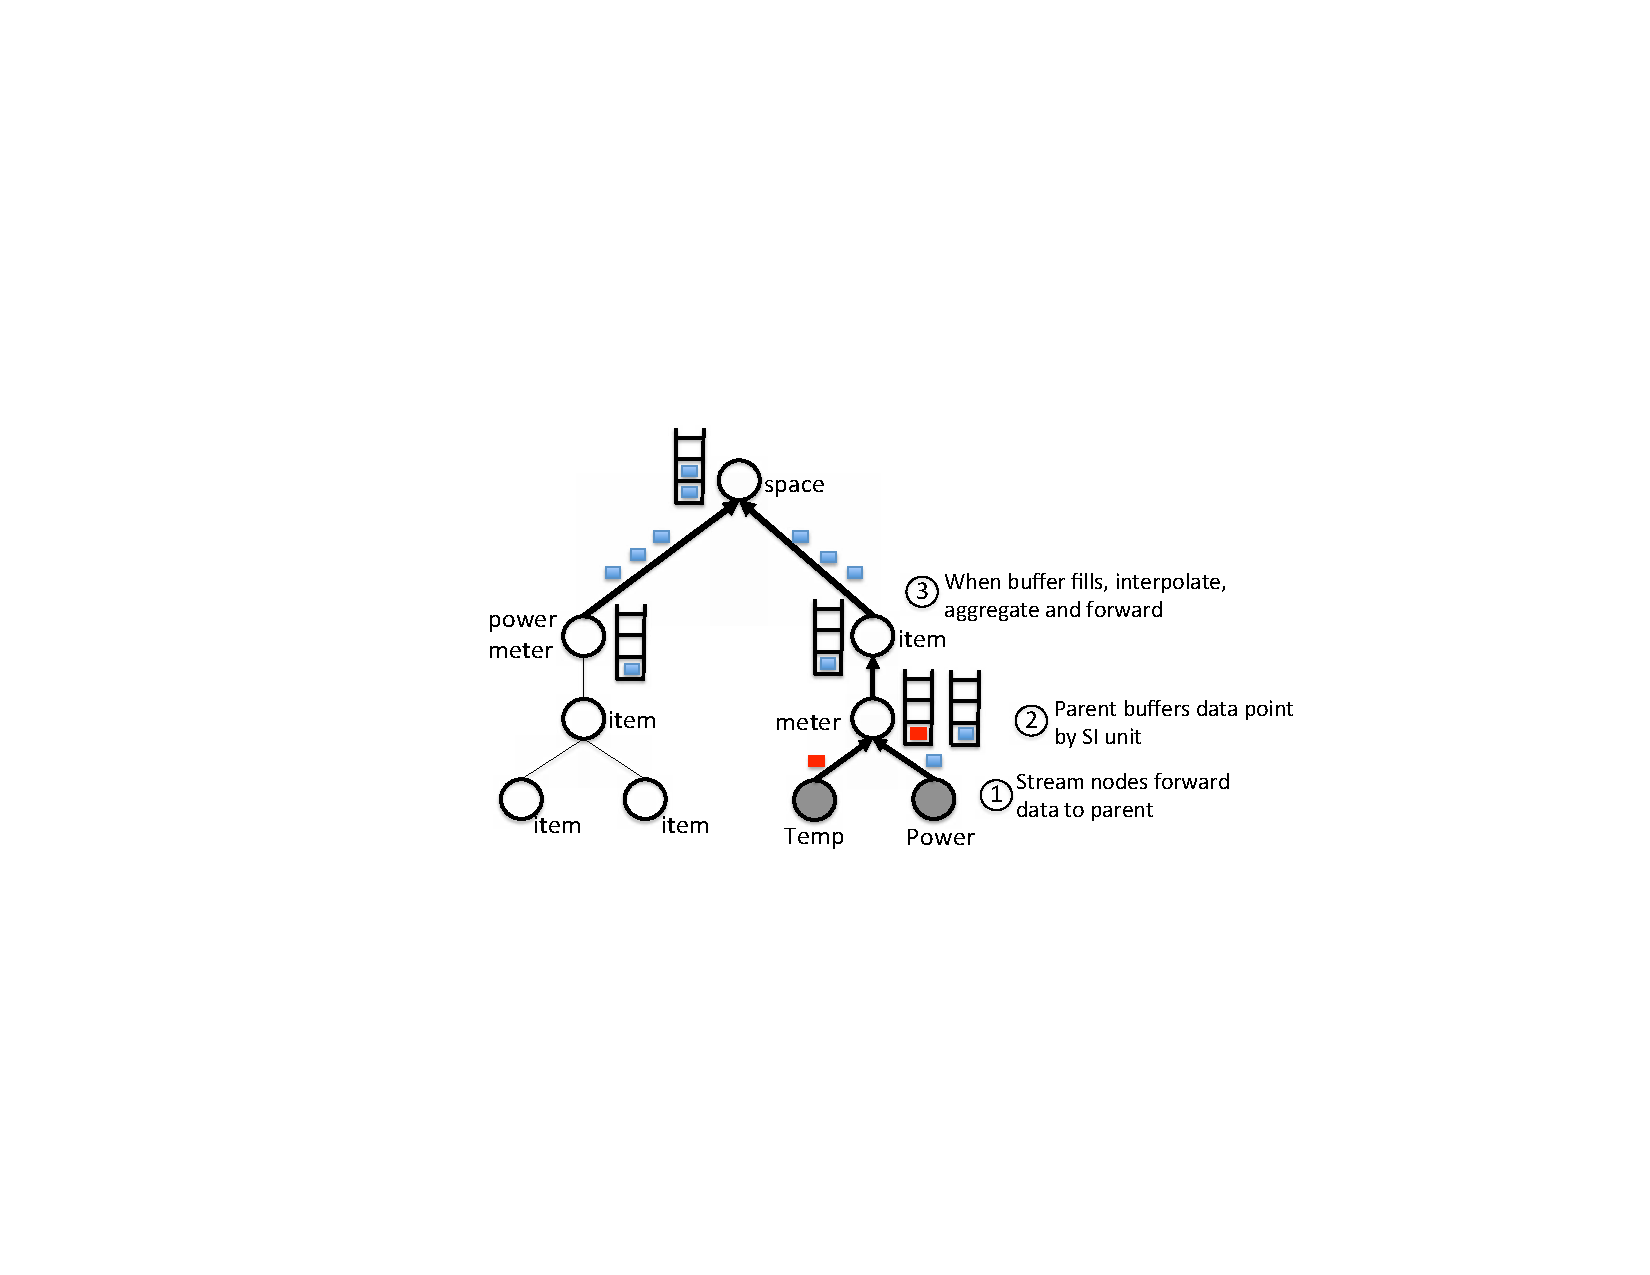
\includegraphics[scale=0.6]{figs/aggtree}
\caption{This shows an illustration of the aggregation tree used by \emph{dynamic aggregation}.  Data flows from 
the leaves to the root through user-specified aggregation points.  When the local buffer is full the streams
are separated by source, interpolated, and summed.  The aggregated signal is foward up the tree.}
\label{fig:aggtree}
\end{center}
\end{figure}

\subsubsection{Dealing with dynamics}
This approach deals with changes in the graph quite naturally.  All aggregation point deal only with local data, so
a node is only concerned about the children that give it data and the parent to send data to.  As objects in the environment
move from place to place and these changes are captured, the entity-relationship graph also changes to reflect the move.
This change in aggregation constituents is naturally accounted for in the aggregate.  If a child is removed,
it no longer forwards data to the old parent, therefore the aggregate will reflect that change.
Note, however, that changes in the entity-relationship graph are indistinguishable from energy-consuming items that have
been turned off.  For the purposes of aggregation, that is okay.

\subsubsection{Two scenarios}
We illustrate dynamic aggregation with a common usage scenario.  Imagine there are a number of people in a building,
each owning a number of plug-load applicances and a laptop.  Assume that when a person is in a room their laptop
is plugged in and when they leave the room they unplug their laptop and take it with them.  People come and go
throughout the day, changing the aggregate power consumption of the room and it happens.  In addition, some
of those people move to other rooms and plug their laptop in the new location.  As this happens, we will assume
all actions are being recorded in StreamFS.

%FILL IN WITH REAL GRAPH
\begin{figure}[htb!]
\begin{center}
\subfloat[Room 1 object and aggregate streams.]{%
            \label{fig:dynaggs1room1}
            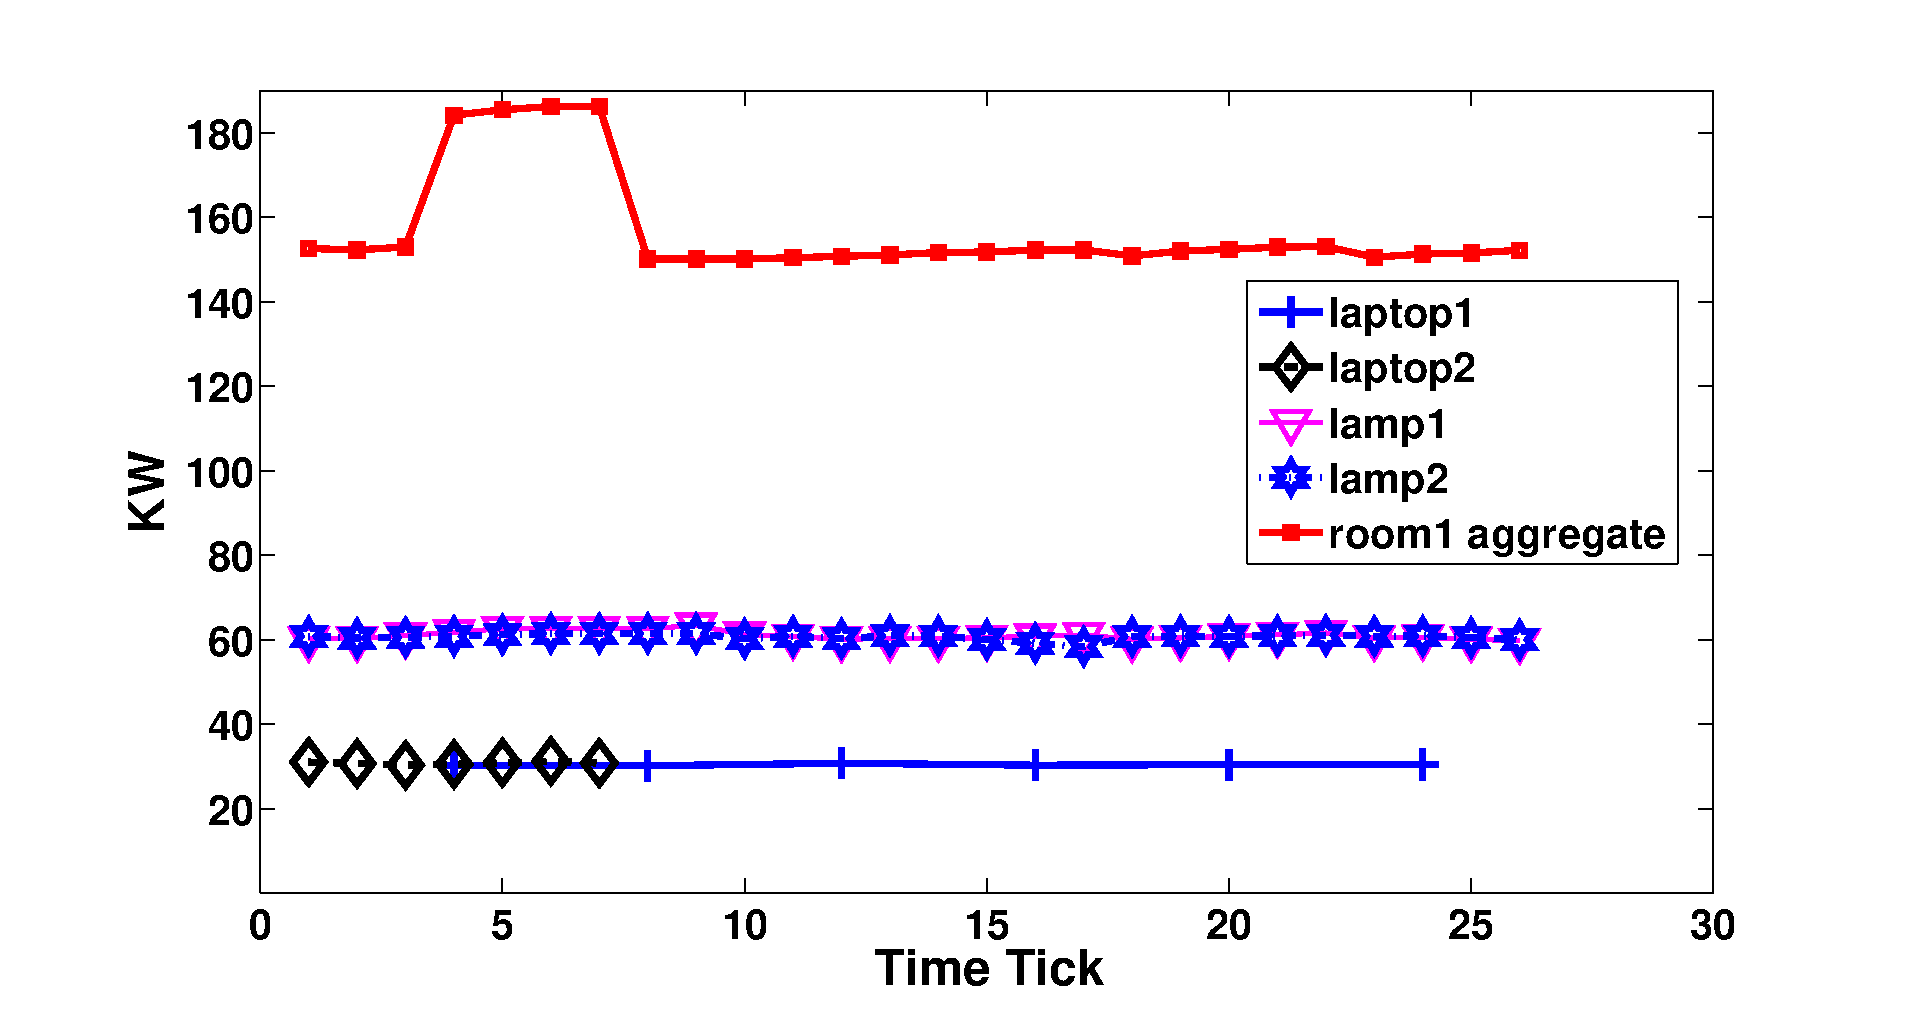
\includegraphics[scale=0.4]{figs/dynagg_scenario1_room1}
        }
\subfloat[Room 2 aggregate.]{%
            \label{fig:dynaggs1room2}
            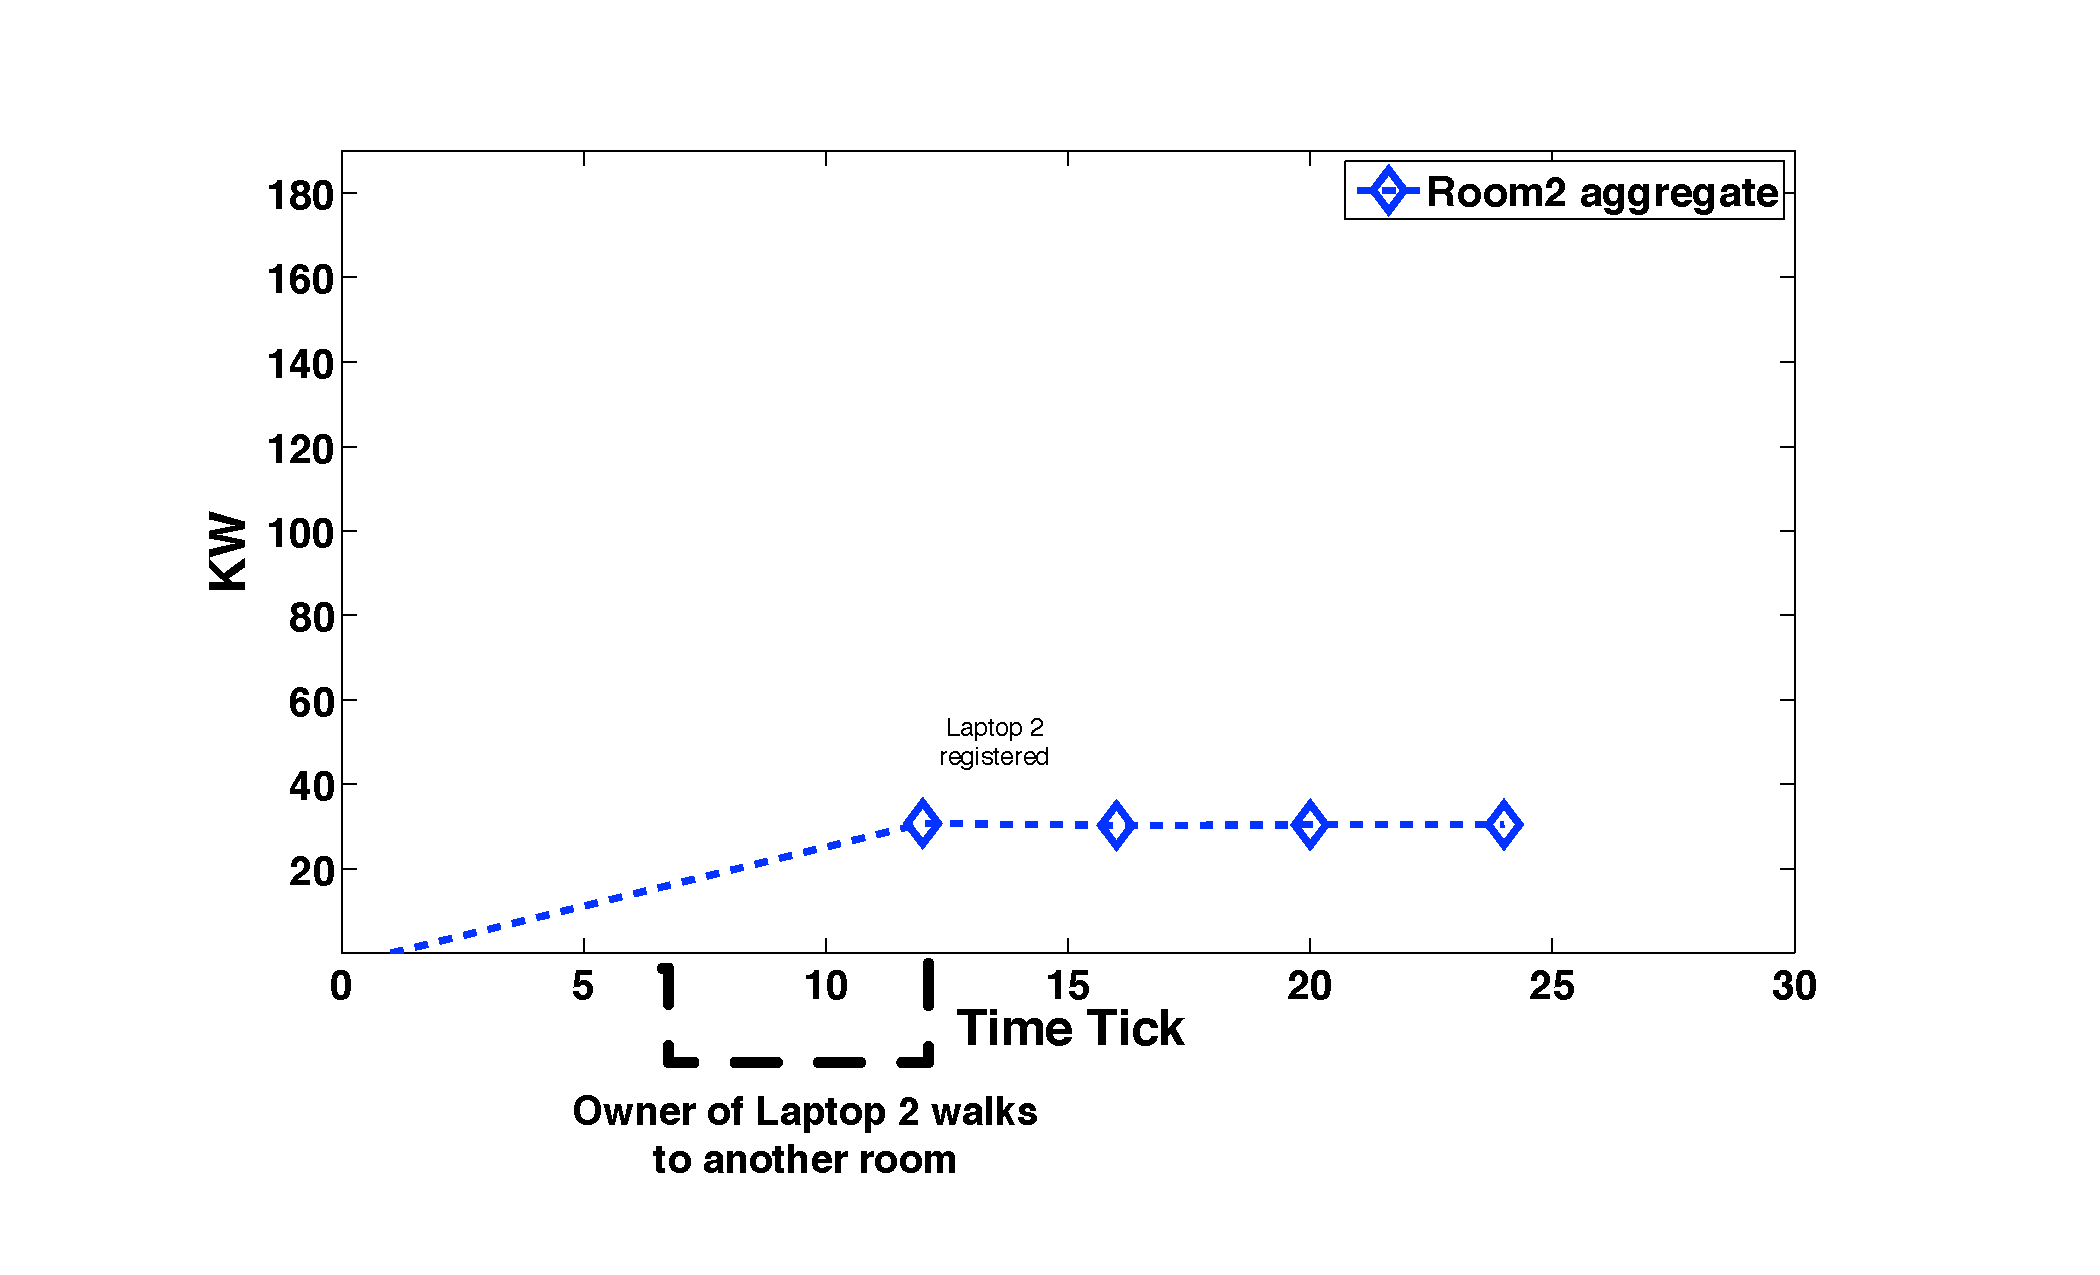
\includegraphics[scale=0.4]{figs/dynagg_scenario1_room2}
        }
\end{center}
\caption{
	The power consumes by a laptop in \emph{room 1} is shifted to \emph{room 2} a time t=7.  Notice the aggregagate drops in room 1
	while it rises in room 2.
     }%
\label{fig:multiroomagg}
\end{figure}

Figure~\ref{fig:multiroomagg} illustrate the aggregation results of that scenario.  Notice how...

% For demonstration lets have the user turn off on of their appliances when they leave as well.  This should cause that total
% room aggregate to drop, the person's personal aggregate to drop, but the other occupant's aggregate to remain
% the same.

% %FILL IN WITH REAL GRAPH
% \begin{figure}[htb!]
% \begin{center}
% 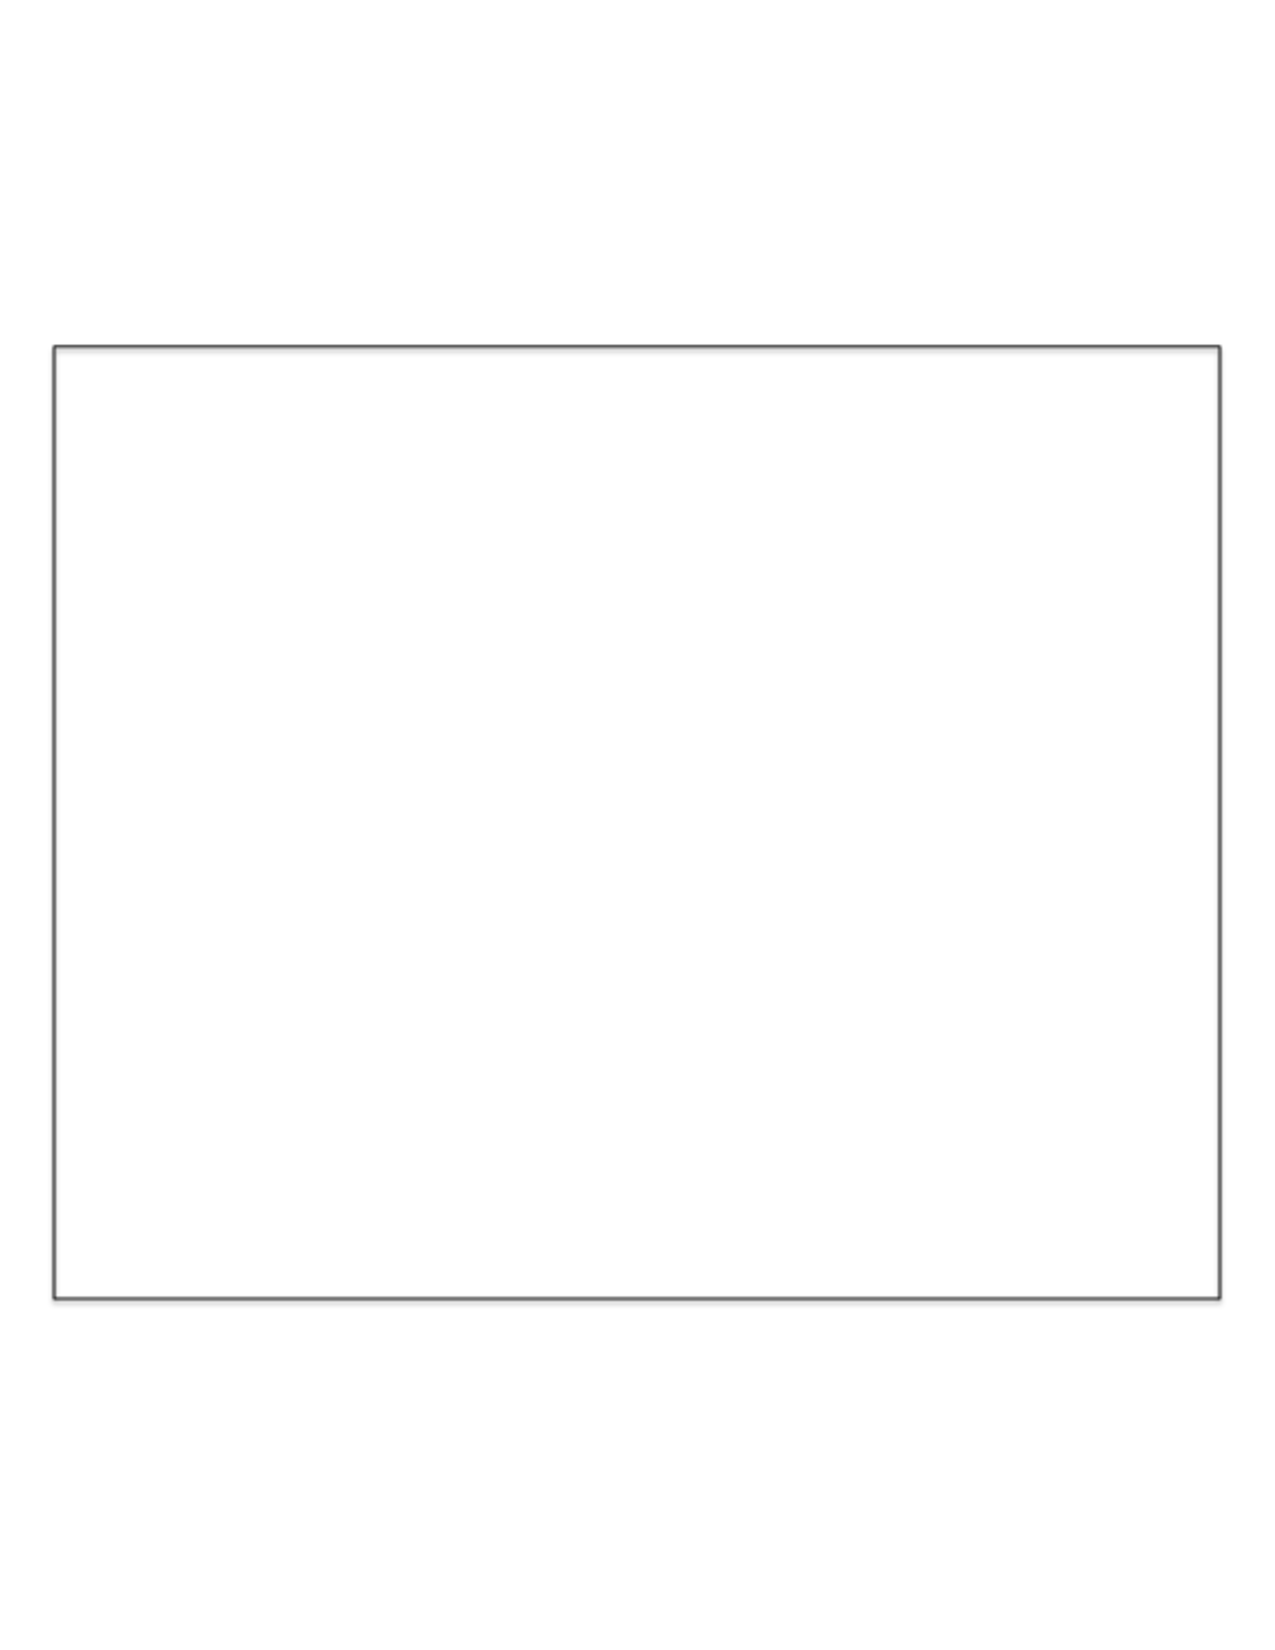
\includegraphics[scale=0.39]{figs/blankbox}
% \caption{A room with items that belong to many users.  Person leaves with their item, aggregate falls.  Show aggregate.
% Person joins another room, aggregate in that room rises.  Show aggregate in the new room.  Compare before and after.}
% \label{fig:personaltotalagg}
% \end{center}
% \end{figure}

% Figure~\ref{fig:personaltotalagg} illustrate the results of the second sceanrio.  Note how...


